\subsection{Procedural Steps}
	\begin{frame}{Procedural Steps}
	\begin{alertblock}{Hypothesis}
		It has been chosen to not use an \textbf{inlet guide vane} for simplicity of design and so $V_{t0} = 0 \frac{m}{s}$ and $\chi$ dictate the behaviour of $\lambda$. Another initial desing choice is to keep, in the similarity/adimensional analysis of the compressor, $V_a$ \textbf{constant} and to \textbf{avoid} using a \textbf{flaring based} approach.
	\end{alertblock}
	\textbf{Main procedural steps:}
	\begin{itemize}
		\item $\lambda$ and $\psi$ computation from $\chi$ and $V_{t0}$
		\item $\phi$ and $\eta$ computation 
		\item $V_a$ and $L_{eu}$ computation from $\phi$, $\beta_{TT}$ and $\eta$
		\item computing \textbf{mean} velocity triangles, using the above hypothesis
		\item computing \textbf{blade height}
	\end{itemize}
	\end{frame}
\subsection{Main Design Quantities}
	\begin{frame}{Graph Analysis: $\chi$ \& $M$}
		\begin{figure}
			\centering
			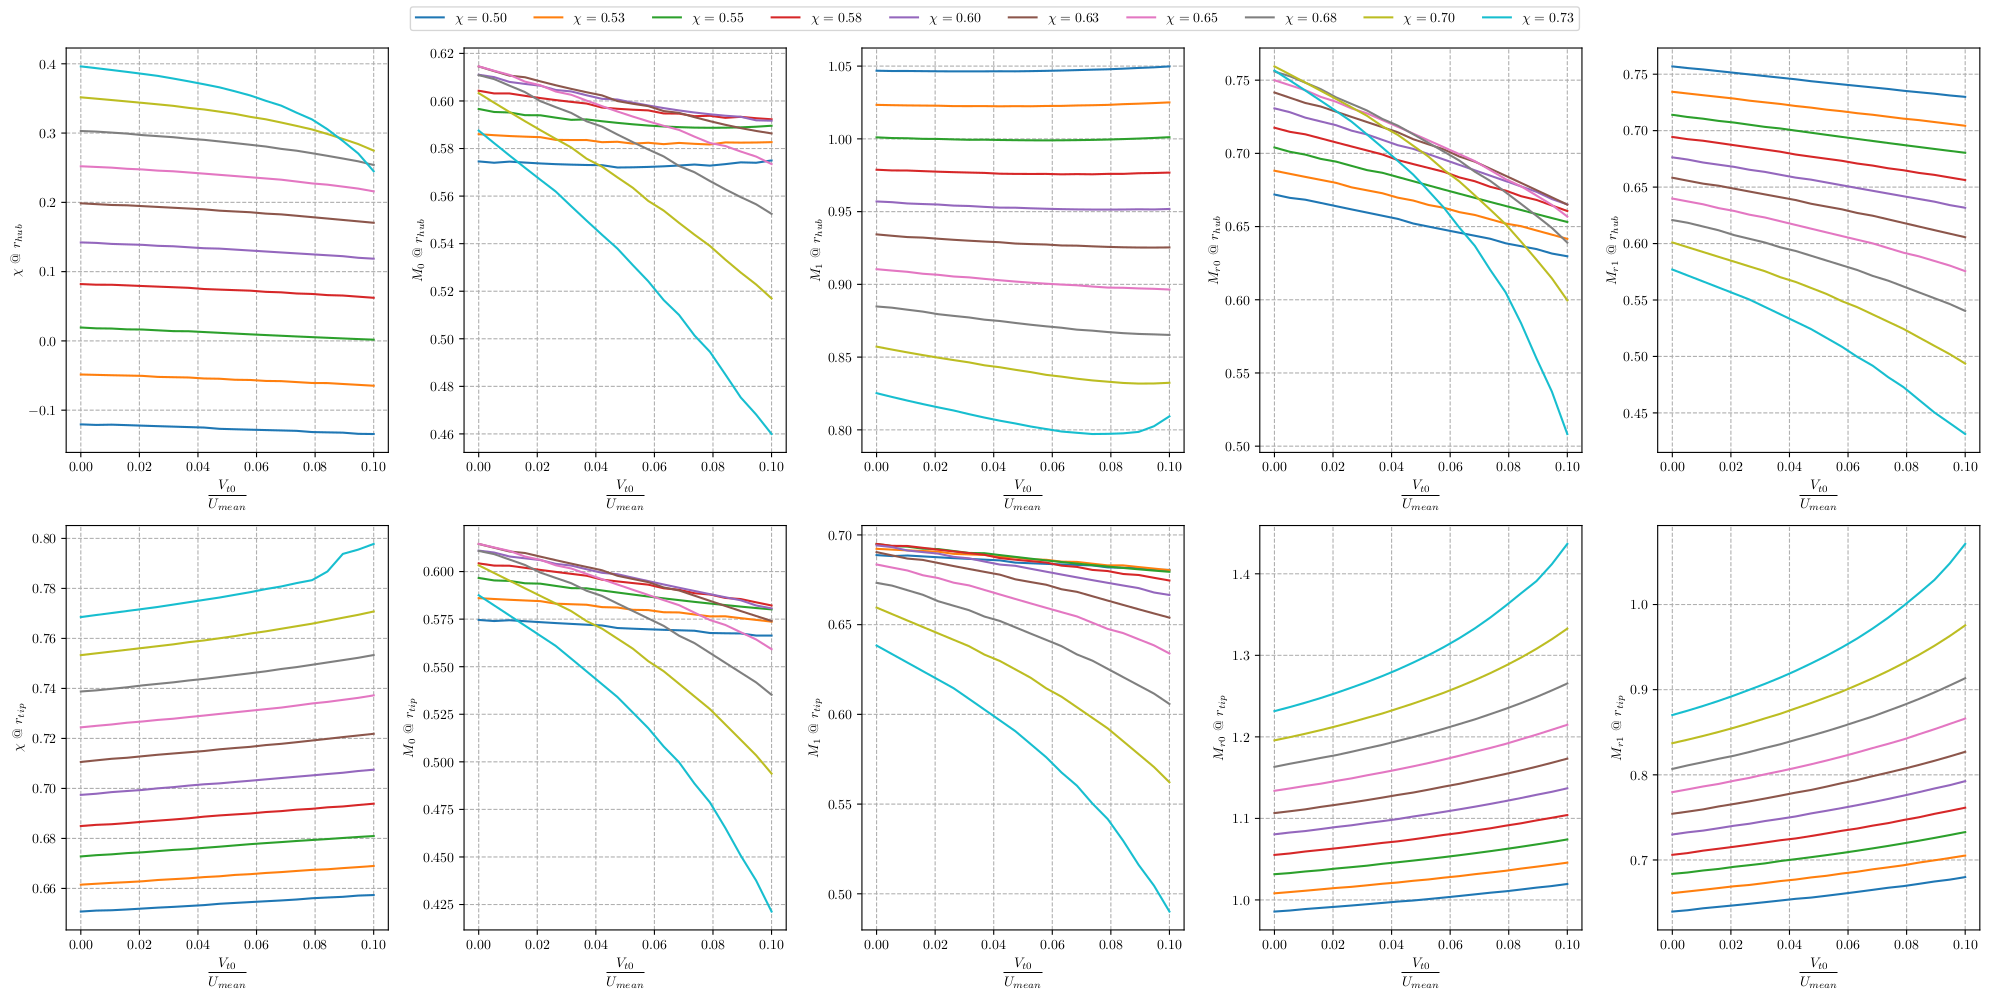
\includegraphics[width=\textwidth]{figures/reactionStudy0.png}
		\end{figure}
	\end{frame}
	\begin{frame}{Graph Analysis: $\alpha$ \& $\beta$}
		\begin{figure}
			\centering
			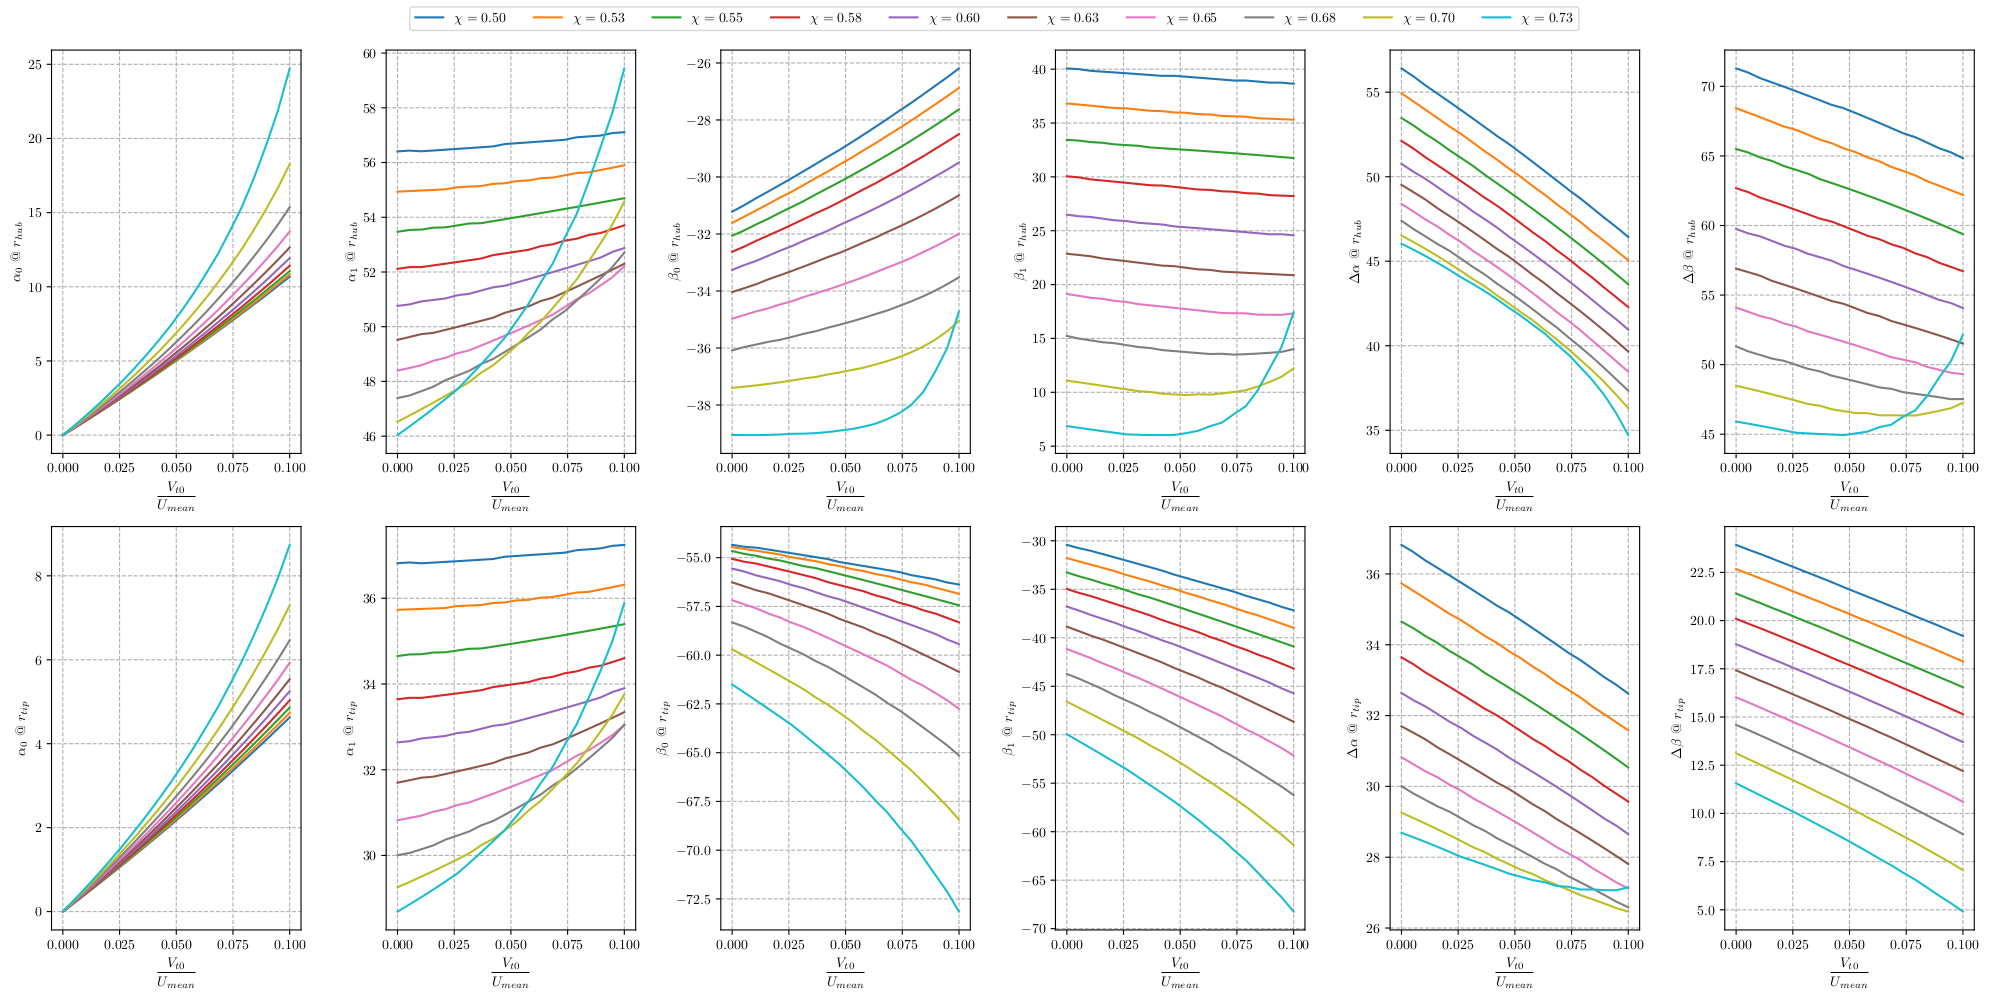
\includegraphics[width=\textwidth]{figures/reactionStudy1.png}
		\end{figure}
	\end{frame}
	\begin{frame}{$\lambda$ \& $\psi$}
		From the previous graphs:
			\begin{itemize}
				\item $\chi = 0.55$
				\item $r_{mean} = 0.325 m$
				\item $\frac{V_t}{U_{mean}} = 0$
			\end{itemize}
		Taking into account the previous modeling hypothesis:
		\begin{align}
			\lambda & = (1 - \chi - \frac{V_t}{U_{mean}}) \cdot 4 \\ 
			\psi    & = \frac{\lambda}{2} 
		\end{align}
	\end{frame}
	
	\begin{frame}{$\phi_{(\psi)}$}
		From \cite[Sec. 10.4]{axial2004} it is imposed that $\frac{W_2}{W_1} \geq 0.7$ with a \textit{safety} margin of $2 \%$.  
		\begin{figure}
			\centering
			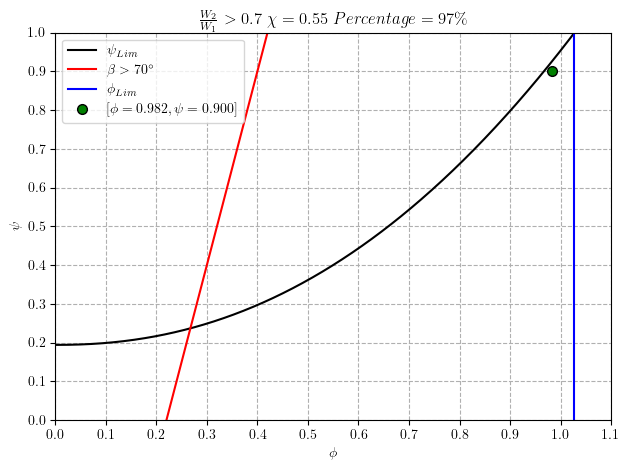
\includegraphics[width=0.7\textwidth]{figures/stagePerf.png}
		\end{figure}
	\end{frame}
	\begin{frame}{$\eta$ \& $L_{eu}$}
		$\eta$ is computed from an \textbf{Lieblein} efficiency chart\footnote{This chart has been interpolated from the course slides charts.} given $\phi$ and $\chi$. This parameter will be used for the computation of $L_{eu}$ given the $\beta_{TT}$ target.
		\begin{columns}
			\column{0.5\textwidth}
				\begin{figure}
					\centering 
					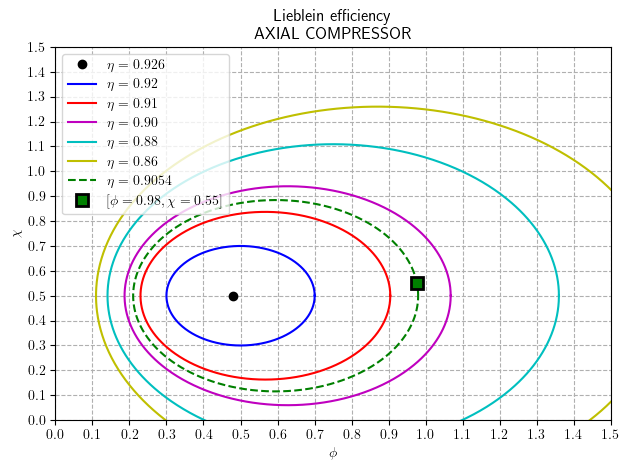
\includegraphics[width=1\textwidth]{figures/efficiency.png}
				\end{figure}
			\column{0.5\textwidth}
			\begin{align}
				L_{is} & = \frac{\gamma \ R}{\gamma - 1} \ T_{in} \ (\beta_{TT}^{{\frac{\gamma - 1}{\gamma}}} - 1) \\
				L_{eu} & = \frac{L_{is}}{\eta}
			\end{align}
		\end{columns}
	\end{frame}
\subsection{$V_{t_{mean}}$, $V_{a_{mean}}$, $U_{mean}$ \& velocity triangles}
\begin{frame}[fragile]
	\begin{align}
		U_{mean} & = \frac{L_{eu}}{\psi} \\ 
		V_{a_{mean}} & = \phi \ U_{mean} \\ 
		L_{eu} & = U_1 \ V_{t1} - U_0 \ V_{t0} \\ 
		       & = U_{1_{mean}} \ V_{t1_{mean}} - U_{0_{mean}} \ V_{t0_{mean}} = U_{mean} \ \Delta V_{t_{mean}} 
	\end{align}
	$\Delta V_t$ computation allows to get a \textit{first sketch} of the \textbf{velocity triangles}.
	The first analysis results are stored in \verb|compressor_0.55_0.325_28_28.txt|.
\end{frame}

{\nologo
\begin{frame}
	\begin{columns}
		\column{0.5\textwidth}
			\begin{figure}
				\centering
				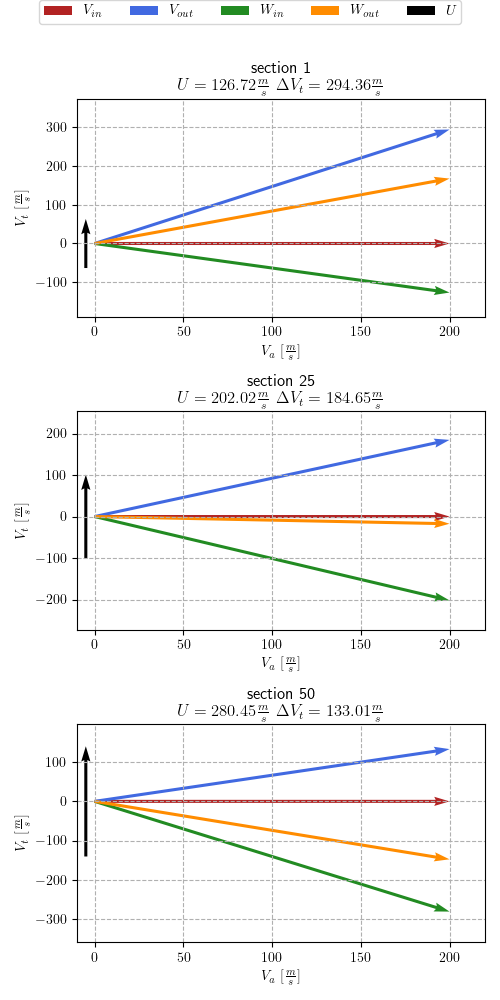
\includegraphics[width=0.7\textwidth]{figures/rotorVelocityTriangle.png}
			\end{figure}
		\column{0.5\textwidth}
			\begin{figure}
				\centering
				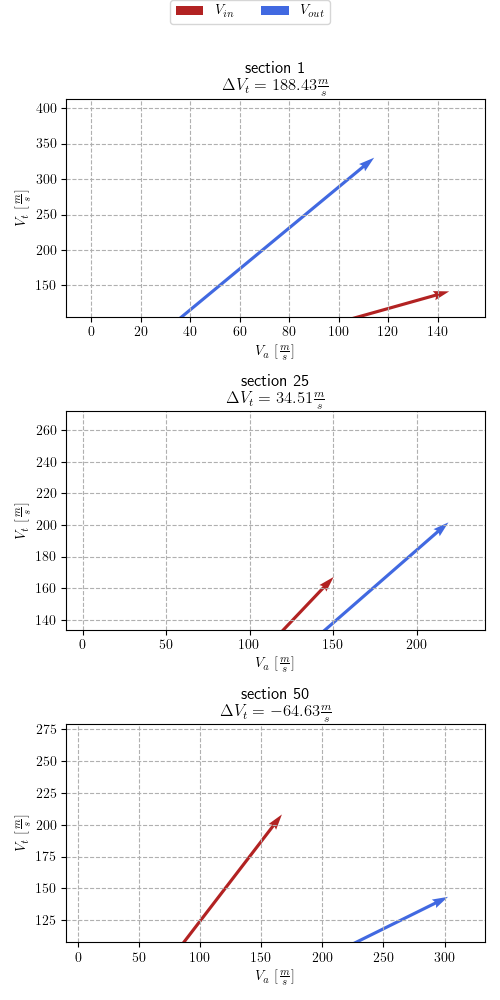
\includegraphics[width=0.7\textwidth]{figures/statorVelocityTriangle.png}
			\end{figure}
	\end{columns}
\end{frame}
}

